\documentclass[11pt,a4paper]{article}
\usepackage[utf8]{inputenc}
\usepackage[spanish]{babel}	%Idioma
\usepackage{amsmath}
\usepackage{amsfonts}
\usepackage{amssymb}
\usepackage{graphicx} 	%Añadir imágenes
\usepackage{geometry}	%Ajustar márgenes
\usepackage[export]{adjustbox}[2011/08/13]
\usepackage{float}
\restylefloat{table}
\usepackage{diagbox}
\usepackage{makecell}
\usepackage[hidelinks]{hyperref}
\usepackage{titling}
%\graphicspath{{/home/nazaret/Escritorio/LaTEX}}
%\usepackage{minted}
\usepackage{multirow}
\usepackage{caption}
\usepackage{multicol}
\usepackage{array}
\selectlanguage{spanish}
\usepackage{xcolor}

%Opciones de encabezado y pie de página:
\usepackage{fancyhdr}
\pagestyle{fancy}
\lhead{Nazaret Román Guerrero}
\rhead{Sistemas Multimedia}
\lfoot{Grado en Ingeniería Informática}
\cfoot{}
\rfoot{\thepage}
\renewcommand{\headrulewidth}{0.4pt}
\renewcommand{\footrulewidth}{0.4pt}

%Opciones de fuente:
\usepackage[utf8]{inputenc}
\usepackage[default]{sourcesanspro}
\usepackage{sourcecodepro}
\usepackage[T1]{fontenc}

\setlength{\parindent}{15pt}
\setlength{\headheight}{15pt}
\setlength{\voffset}{10mm}

% Custom colors
\usepackage{color}
\definecolor{deepblue}{rgb}{0,0,0.5}
\definecolor{deepred}{rgb}{0.6,0,0}
\definecolor{deepgreen}{rgb}{0,0.5,0}

\usepackage{listings}

\begin{document}
\begin{titlepage}

\begin{minipage}{\textwidth}

\centering

\includegraphics[width=0.5\textwidth]{logo.png}\\

\textsc{\Large Sistemas Multimedia\\[0.2cm]}
\textsc{GRADO EN INGENIERÍA INFORMÁTICA}\\[1cm]

{\Huge\bfseries Imagen\\}
\noindent\rule[-1ex]{\textwidth}{3pt}\\[3.5ex]
{\large\bfseries Trabajo voluntario}
\end{minipage}

\vspace{1.5cm}
\begin{minipage}{\textwidth}
\centering

\textbf{Autora}\\ {Nazaret Román Guerrero}\\[2.5ex]

\includegraphics[width=0.3\textwidth]{etsiit.jpeg}\\[0.1cm]
\vspace{1cm}
\textsc{Escuela Técnica Superior de Ingenierías Informática y de Telecomunicación}\\
\vspace{1cm}
\textsc{Curso 2018-2019}
\end{minipage}
\end{titlepage}

\pagenumbering{gobble}
\pagenumbering{arabic}
\tableofcontents
\thispagestyle{empty}

\newpage

\section{Parámetros}

Vamos a comparar distintas imágenes, 7 imágenes concretamente. Para ello, utilizaremos diferentes \textit{códecs}, y, en el caso de que éste lo permita, variaremos algunos parámetros como la compresión. Usaremos las siguientes imágenes, todas en formatos sin compresión (\textsc{.dng} las 4 primeras, \textsc{.bmp} las 3 últimas).

\begin{enumerate}
	\item Imagen con pocos colores (\textsc{poco\_crom.dng}).
	\item Imagen con mucha riqueda cromática (\textsc{crom.dng}).
	\item Imagen de una persona (\textsc{retrato.dng}).
	\item Imagen con pocas texturas (\textsc{pocas\_texturas.dng}).
	\item Imagen con muchas texturas (\textsc{texturas.dng}).
	\item Imagen con texto (\textsc{texto.bmp}).
	\item Imagen gráfica (\textsc{graficos.bmp}).
\end{enumerate}

Para cada imagen, crearemos una tabla con cada \textit{códec} en una fila y tres columnas indicando el tamaño de la imagen, la valoración que se le da, y la posición en el ranking. Para la valoración se utilizarán iconos, descritos más abajo.\\

Además, para los \textsc{códecs} que admitan compresión, habrá más filas correspondientes a dicha compresión. Para las imágenes en \textsc{jpeg}, para hablar de compresión hablaremos de ``calidad'', un valor que estará entre 1 y 100 (donde 1 es máxima compresión y peor calidad, y 100 es máxima calidad pero nada de compresión). Para las imágenes en \textsc{tiff} simplemente hablaremos de compresión, y será uno de entre los dos siguientes: sin compresión o compresión con deflación.\\

Los iconos que se van a utilizar para las valoraciones son:

\begin{itemize}
	\item Muy buena = 
\includegraphics[width=0.05\textwidth]{mb.png}
	\item Buena = 
\includegraphics[width=0.05\textwidth]{b.png}
	\item Regular = 
\includegraphics[width=0.05\textwidth]{r.png}
	\item Mala = 
\includegraphics[width=0.05\textwidth]{m.png}
	\item Muy mala = 
\includegraphics[width=0.05\textwidth]{mm.png}
\end{itemize}


\subsection{Imagen con pocos colores}

Esta primera imagen, mostrada debajo, utilizaremos una imagen tomada de un manga, los cuales son impresos en escala de grises.

\begin{itemize}
	\item Formato original: \textsc{.dng}
	\item Tipo de imagen: poco cromática
	\item Imagen:
		\begin{figure}[H]
		\centering
			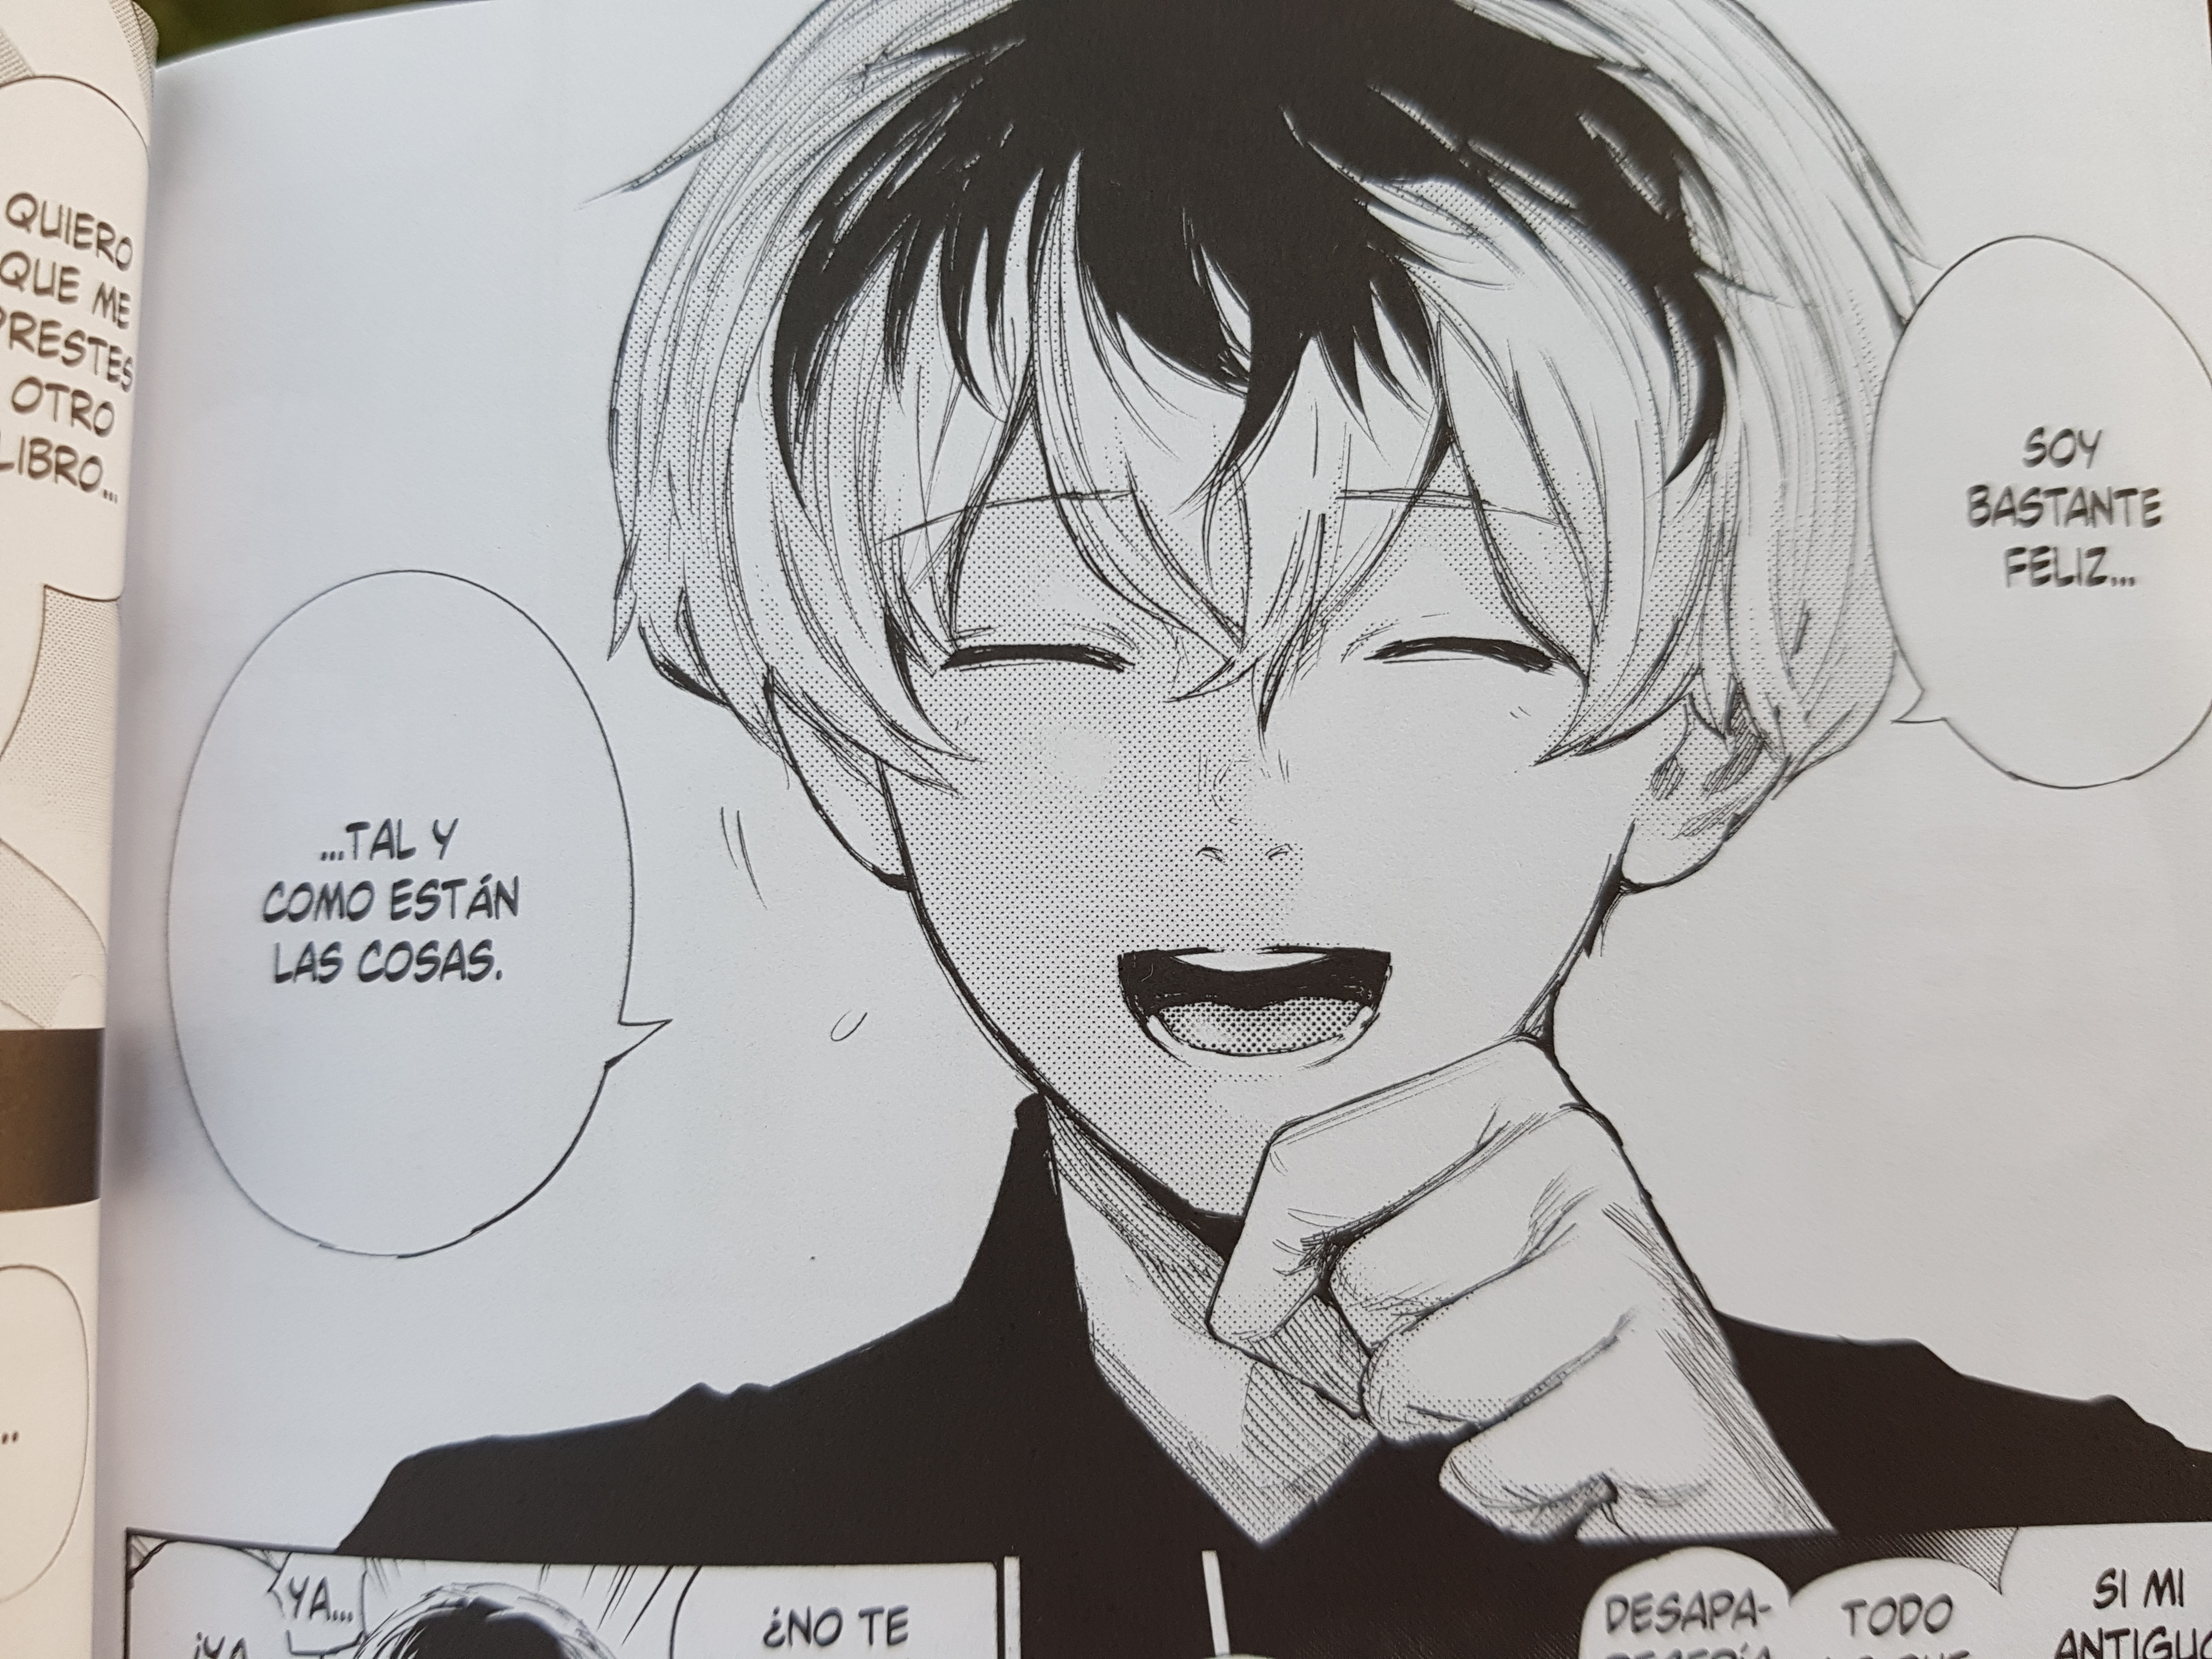
\includegraphics[width=0.5\textwidth]{Fotos/poco_crom.jpg}
		\end{figure}	
\end{itemize}

\begin{table}[H]
\centering
\begin{tabular}{|c|c|c|c|}
\hline
\diagbox[width=15em]{\textit{Códec}/Formato}{\\Información} & Tamaño & Valoración & Ranking \\
\hline
\textsc{bmp} & 36.4 MB & 
\includegraphics[width=0.03\textwidth]{mb.png} & 1º \\ \hline
\textsc{tiff} sin compresión & 36.6 MB & 
\includegraphics[width=0.03\textwidth]{b.png} & 2º \\ \hline
\textsc{tiff} con deflación & 29.2 MB & 
\includegraphics[width=0.03\textwidth]{b.png} & 2º \\ \hline
\textsc{gif} & 9.7 MB & 
\includegraphics[width=0.03\textwidth]{mb.png} & 1º \\ \hline
\textsc{jpeg} con calidad :100 & 17.3 MB & 
\includegraphics[width=0.03\textwidth]{b.png} &  2º \\ \hline
\textsc{jpeg} con calidad :50 & 731.9 kB & 
\includegraphics[width=0.03\textwidth]{b.png} &  2º \\ \hline
\textsc{jpeg} con calidad :5 & 144 kB & 
\includegraphics[width=0.03\textwidth]{mm.png} & 3º \\ \hline
\textsc{png} & 22.4 MB & 
\includegraphics[width=0.03\textwidth]{b.png} & 2º \\ \hline
\end{tabular}
\caption{Imagen poco cromática}
\label{tab:my-table}
\end{table}

\subsubsection{Explicaciones a las valoraciones}
\begin{enumerate}
	\item \textsc{bmp} y \textsc{gif}: en esta primera imagen, dan los mejores resultados debido a que la imagen debe verse en blanco y negro y no en escalas de gris. Por tanto, estos formatos que tienen menos profundidad de color hacen que la imagen se vea mucho mejor que en el resto de casos.
	\item \textsc{tiff} sin compresión y con deflación, \textsc{jpeg} con calidad 100 y 50 y \textsc{png}: la imagen se ve bien, pero se introduce ruido, ya que los tonos que deberían ser negros se ven de una tonalidad oscura de gris. Teniendo en cuenta cómo debe ser esta imagen en concreto, con estos \textit{códecs} se ve peor que con los dos anteriores.
	\item \textsc{jpeg} con calidad 5: no solo esta imagen introduce ruido, sino que además se ven múltiples ``manchas'' por toda la imagen, ya que al comprimir más, los pixeles toman los valores de alrededor y parece una imagen con parches. Se pierde mucha calidad respecto a los demás \textit{códecs}.
\end{enumerate}

\subsubsection{Conclusión}

En esta imagen del manga de \textit{Tokyo Ghoul:re}, en escala de grises, aquellos \textit{códecs} que permiten menos profundidad de color, es decir, que tienen menos variedad de color (y por tanto menos tonos de gris), hace que los colores se marquen mejor ya que la finalidad de un manga es que se vea en blanco o negro. Por tanto, se aprecian mejor estos colores en \textsc{.gif} y \textsc{.bmp}

\newpage

\subsection{Imagen con muchos colores}

Esta imagen fue tomada en un parque con flores y vegetación, tiene una gran variedad de colores.

\begin{itemize}
	\item Formato original: \textsc{.dng}
	\item Tipo de imagen: muy cromática
	\item Imagen:
		\begin{figure}[H]
		\centering
			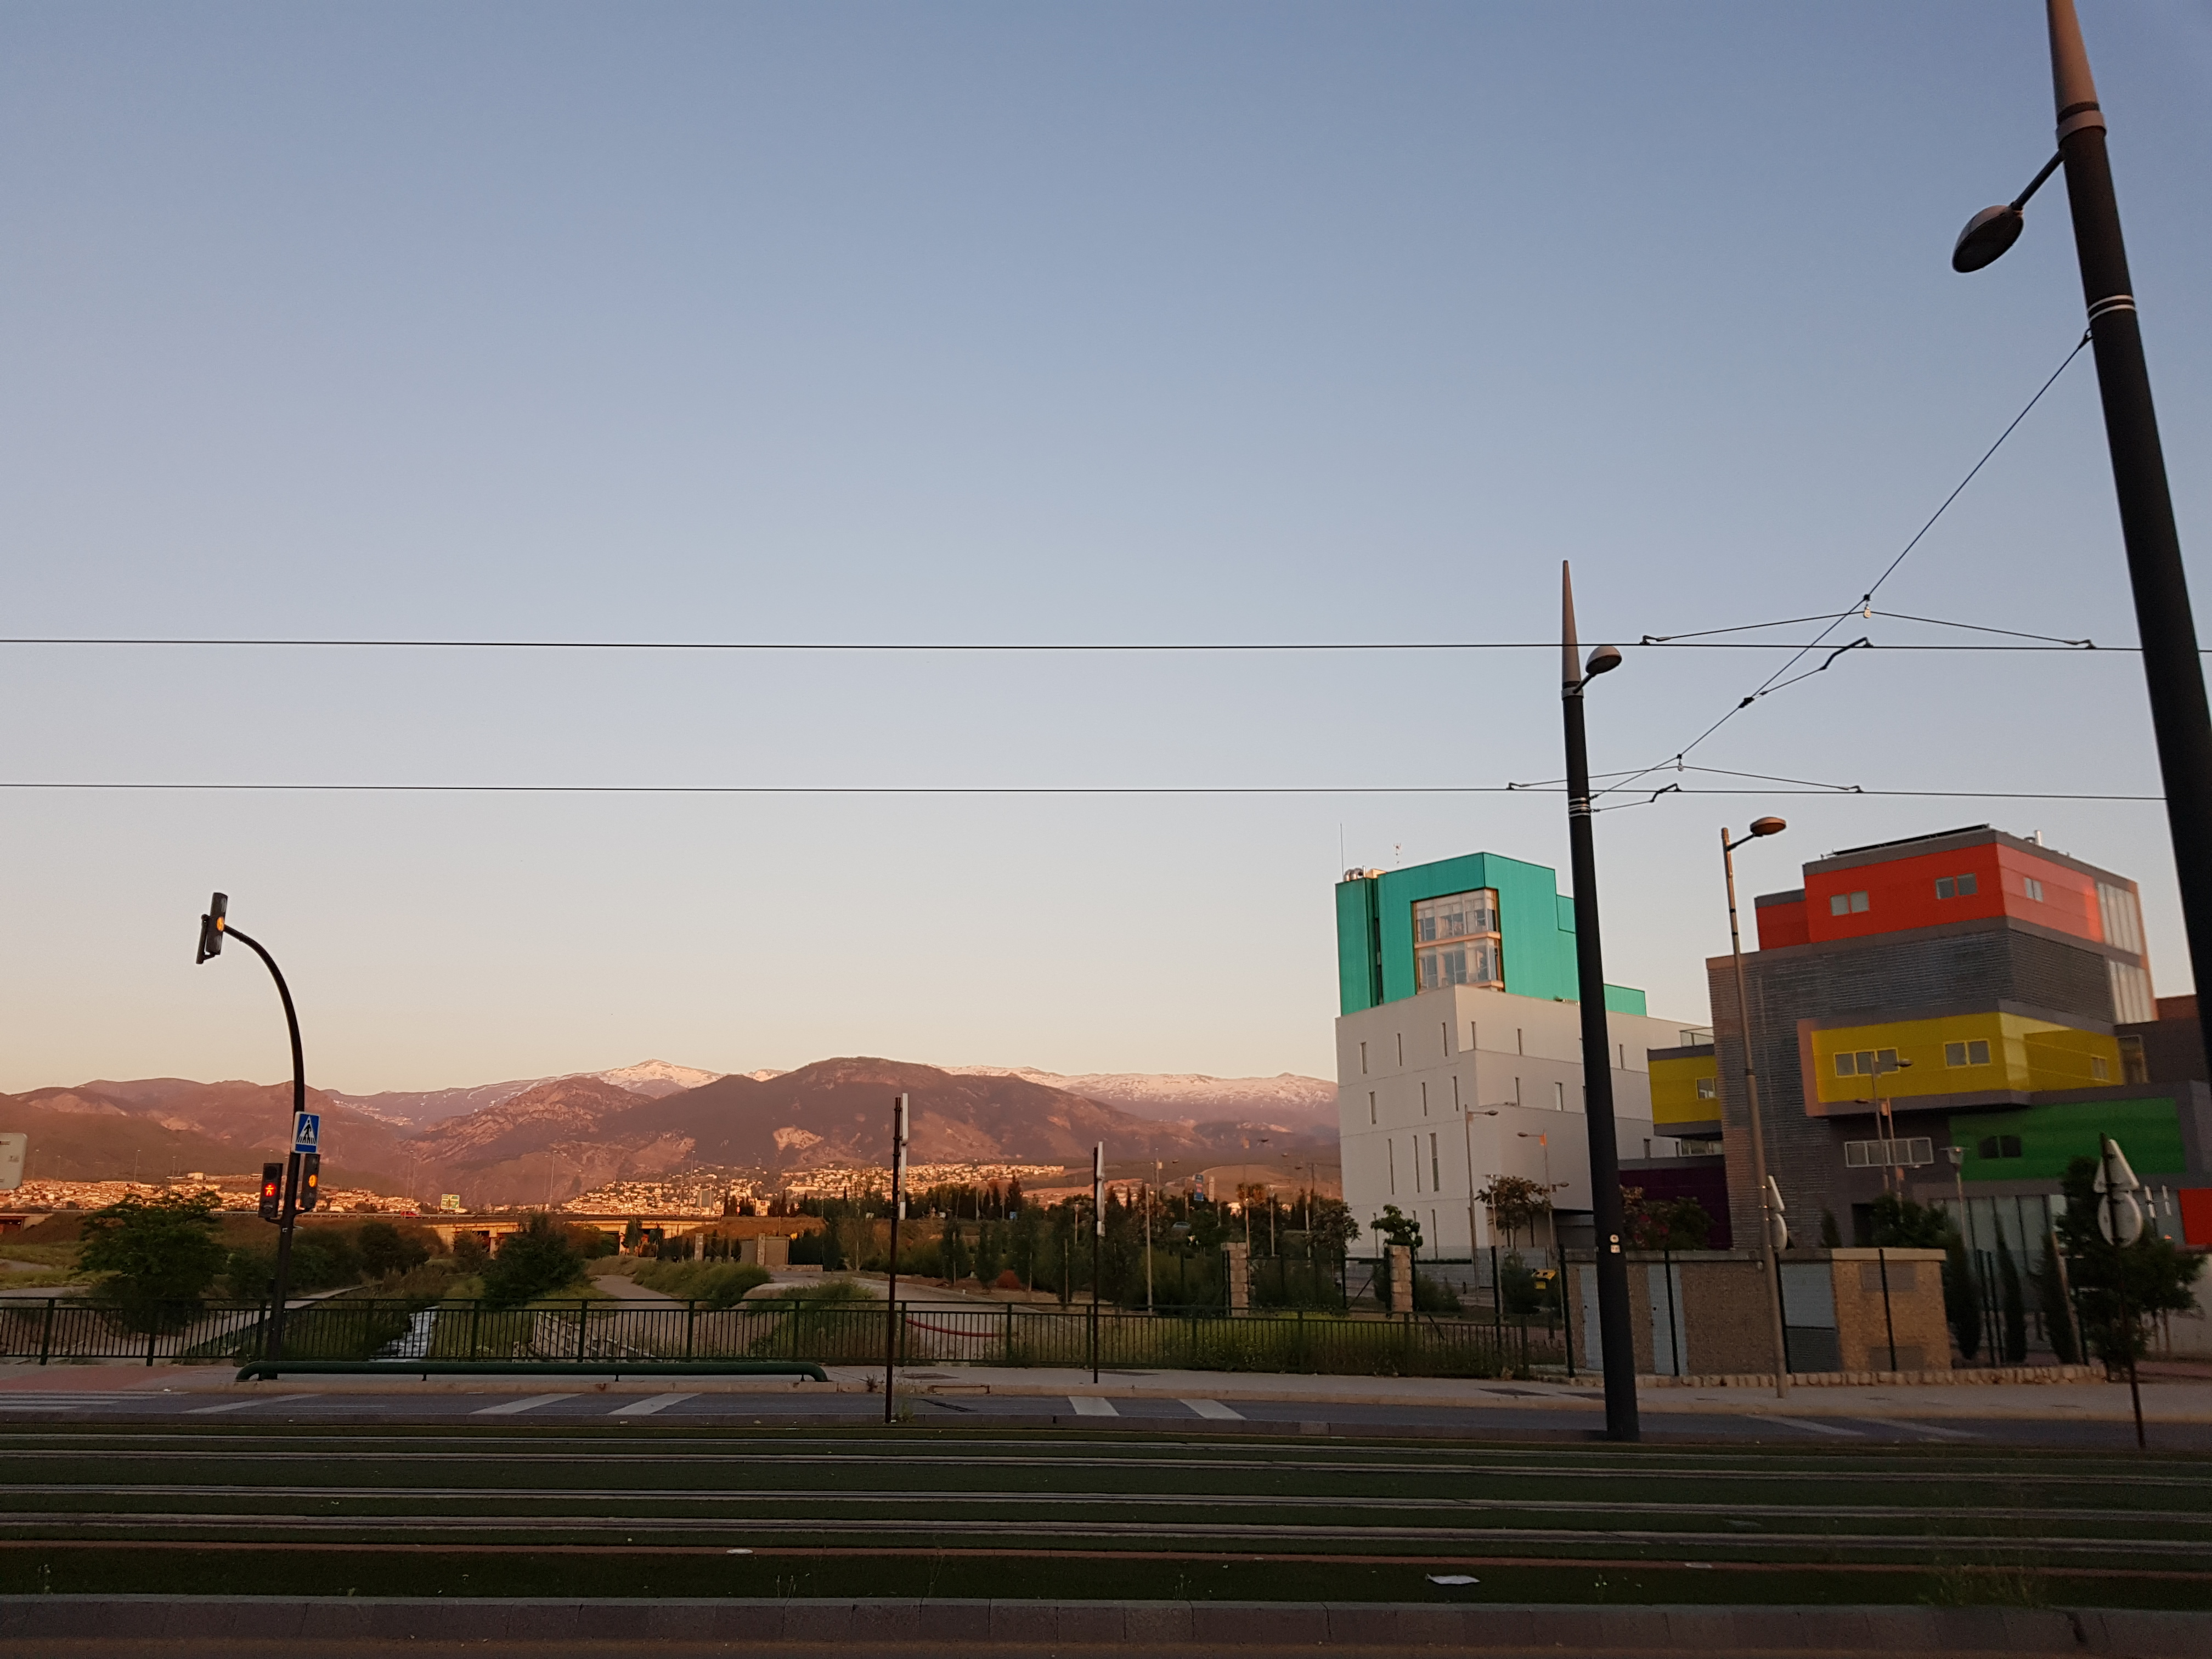
\includegraphics[width=0.5\textwidth]{Fotos/crom.jpg}
		\end{figure}	
\end{itemize}

\begin{table}[H]
\centering
\begin{tabular}{|c|c|c|c|}
\hline
\diagbox[width=15em]{\textit{Códec}/Formato}{\\Información} & Tamaño & Valoración & Ranking \\
\hline
\textsc{bmp} & 36.4 MB & 
\includegraphics[width=0.03\textwidth]{r.png} & 3º \\ \hline
\textsc{tiff} sin compresión & 36.6 MB & 
\includegraphics[width=0.03\textwidth]{mb.png} & 1º \\ \hline
\textsc{tiff} con deflación & 29.5 MB & 
\includegraphics[width=0.03\textwidth]{mb.png} & 1º \\ \hline
\textsc{gif} & 8.1 MB & 
\includegraphics[width=0.03\textwidth]{r.png} & 3º \\ \hline
\textsc{jpeg} con calidad :100 & 36.4 MB & 
\includegraphics[width=0.03\textwidth]{mb.png} & 1º \\ \hline
\textsc{jpeg} con calidad :50 & 22.4 MB & 
\includegraphics[width=0.03\textwidth]{mb.png} & 1º \\ \hline
\textsc{jpeg} con calidad :5 & 328.7 kB & 
\includegraphics[width=0.03\textwidth]{mm.png} & 4º \\ \hline
\textsc{png} & 27.1 MB & 
\includegraphics[width=0.03\textwidth]{b.png} & 2º \\ \hline
\end{tabular}
\caption{Imagen poco cromática}
\label{tab:my-table}
\end{table}

\subsubsection{Explicaciones a las valoraciones}
\begin{enumerate}
	\item \textsc{tiff} sin compresión y con deflación, \textsc{jpeg} con calidad 100 y 50: la imagen se ve perfecta, se aprecian todas las tonalidades fieles a la realidad y sin que se introduzca ruido en la imagen.
	\item \textsc{png}: la imagen se ve muy bien, al igual que con los anteriores; no obstante, hay algunas tonalidades (las de las flores rojas por ejemplo) que se ven algo más claras al acercar la imagen. Pero aún así, la imagen a simple vista se ve perfecta.
	\item \textsc{bmp} y \textsc{gif}: con estos formatos sí se ven muchas diferencias respecto a la imagen real, ya que cambian todos los colores y se pierde casi la parte de la imagen más oscura, en los árboles de la izquierda, donde, con estos \textit{códecs} se deja de ver con nitidez y claridad qué hay ahí.
	\item \textsc{jpeg} con calidad 5: con esta compresión se pierde toda la calidad original. Se ven ``cuadraditos'' por toda la imagen y se aprecia por ejemplo la forma de las flores ya que se ven pixeladas.
\end{enumerate}

\subsubsection{Conclusión}

Para esta imagen, son mucho mejores los \textit{códecs} que tienen una gran profundidad de colores y que mantienen la calidad, comprimiendo sin pérdidas o con pérdidas pero no excesivas. Por eso en el ranking los \textit{códecs} como \textsc{jpeg}, \textsc{tiff} o \textsc{png} son los que mejor se ven.

\newpage

\subsection{Retrato}

En este caso, trataremos una imagen de una persona.

\begin{itemize}
	\item Formato original: \textsc{.dng}
	\item Tipo de imagen: retrato
	\item Imagen:
		\begin{figure}[H]
		\centering
			
\includegraphics[width=0.5\textwidth]{Fotos/retrato.jpg}
		\end{figure}	
\end{itemize}

\begin{table}[H]
\centering
\begin{tabular}{|c|c|c|c|}
\hline
\diagbox[width=15em]{\textit{Códec}/Formato}{\\Información} & Tamaño & Valoración & Ranking \\
\hline
\textsc{bmp} & 36.4 MB & 
\includegraphics[width=0.03\textwidth]{r.png} & 3º \\ \hline
\textsc{tiff} sin compresión & 36.6 MB & 
\includegraphics[width=0.03\textwidth]{b.png} & 2º \\ \hline
\textsc{tiff} con deflación & 33.3 MB & 
\includegraphics[width=0.03\textwidth]{mb.png} & 1º \\ \hline
\textsc{gif} & 9.2 MB & 
\includegraphics[width=0.03\textwidth]{r.png} & 3º \\ \hline
\textsc{jpeg} con calidad :100 & 19 MB & 
\includegraphics[width=0.03\textwidth]{b.png} & 2º \\ \hline
\textsc{jpeg} con calidad :50 & 729 kB & 
\includegraphics[width=0.03\textwidth]{mb.png} & 1º \\ \hline
\textsc{jpeg} con calidad :5 & 104 kB & 
\includegraphics[width=0.03\textwidth]{mm.png} & 4º \\ \hline
\textsc{png} & 23.7 MB & 
\includegraphics[width=0.03\textwidth]{b.png} & 2º \\ \hline
\end{tabular}
\caption{Imagen poco cromática}
\label{tab:my-table}
\end{table}

\subsubsection{Explicaciones a las valoraciones}
\begin{enumerate}
	\item \textsc{tiff} con deflación y \textsc{jpeg} con calidad 50: con mi subjetiva opinión, la imagen en con estos \textit{códecs} se ve mejor, ya que se eliminan brillos (como los de la nariz) que hacen que los rasgos se vean mejor definidos, ya que se quita parte del ``haz'' de luz.
	\item \textsc{tiff} sin compresión, \textsc{jpeg} con calidad 100 y \textsc{png}: por sorprendente que parezca, estos \textit{códecs} mantienen la luz que le da al rostro y hacen que los rasgos faciales se vean menos definidos, ya que se eliminan sombras que dan profundidad (se ve especialmente en la nariz).
	\item \textsc{bmp} y \textsc{gif}: en estos casos, la imagen se ve peor, ya que todos los colores se ven oscurecidos. El pelo y la piel se ven mucho más oscuros, por lo que, aunque se mantenga nitidez y se aprecien bien los rasgos, se ha perdido riqueza de color.
	\item \textsc{jpeg} con calidad 5: al igual que en las imágenes anteriores, se ven cuadrados de un mismo color por toda la imagen y se pierden todos los detalles, como por ejemplo el color de ojos; se pierde toda la nitidez, la calidad es muy mala.
\end{enumerate}

\subsubsection{Conclusión}

En esta imagen, a pesar de que lo lógico hubiese sido que los formatos sin pérdidas se viesen mejor, en este caso no es así, ya que el hecho de perder intensidad de la luz hace que el contorno de las partes de la cara se vean mejor definidas, lo que hace que el aspecto visual de la imagen sea más nítido.

\newpage

\subsection{Imagen con pocas texturas}

La imagen que vamos a modificar ahora está sacada de un tablón de madera que forma parte de la puerta de un armario.

\begin{itemize}
	\item Formato original: \textsc{.dng}
	\item Tipo de imagen: poco texturizada
	\item Imagen:
		\begin{figure}[H]
		\centering
			
\includegraphics[width=0.5\textwidth]{Fotos/pocas_texturas.jpg}
		\end{figure}	
\end{itemize}

\begin{table}[H]
\centering
\begin{tabular}{|c|c|c|c|}
\hline
\diagbox[width=15em]{\textit{Códec}/Formato}{\\Información} & Tamaño & Valoración & Ranking \\
\hline
\textsc{bmp} & 36.4 MB & 
\includegraphics[width=0.03\textwidth]{b.png} & 2º \\ \hline
\textsc{tiff} sin compresión & 36.6 MB & 
\includegraphics[width=0.03\textwidth]{mb.png} & 1º \\ \hline
\textsc{tiff} con deflación & 29.9 MB & 
\includegraphics[width=0.03\textwidth]{mb.png} & 1º \\ \hline
\textsc{gif} & 10.8 MB & 
\includegraphics[width=0.03\textwidth]{b.png} & 2º \\ \hline
\textsc{jpeg} con calidad :100 & 19.2 MB & 
\includegraphics[width=0.03\textwidth]{mb.png} & 1º \\ \hline
\textsc{jpeg} con calidad :50 & 694.3 kB & 
\includegraphics[width=0.03\textwidth]{mb.png} & 1º \\ \hline
\textsc{jpeg} con calidad :5 & 95.3 kB & 
\includegraphics[width=0.03\textwidth]{mm.png} & 3º \\ \hline
\textsc{png} & 23.7 MB & 
\includegraphics[width=0.03\textwidth]{mb.png} & 1º \\ \hline
\end{tabular}
\caption{Imagen poco cromática}
\label{tab:my-table}
\end{table}

\subsubsection{Explicaciones a las valoraciones}
\begin{enumerate}
	\item \textsc{tiff} sin compresión y con deflación, \textsc{jpeg} con calidad 100 y 50 y \textsc{png}: la calidad y los colores originales se conservan, es nítida y se ve muy bien.
	\item \textsc{bmp} y \textsc{gif}: de nuevo, muy nítida y con la calidad original, pero en estos dos casos, los colores se oscurecen bastante, por lo que la madera parece de otro tipo. No obstante, se siguen apreciando todos los detalles del veteado de la madera.
	\item \textsc{jpeg} con calidad 5: al igual que en todo los casos de imágenes anteriores, la imagen se ve pixelada, con colores violetas en la parte donde la madera recibe más luz incluso. No conserva nada de calidad.
\end{enumerate}

\subsubsection{Conclusión}

En una imagen con pocos cambios de color y de textura como ha sido ésta, casi cualquier \textit{códec} que utilicemos va a hacer que la imagen consiga mantener su calidad y todos sus colores originales. Si bien es cierto que se puede ver más oscura o más clara dependiendo de la profundidad de color que acepte el \textit{códec}, los detalles se han mantenido iguales en casi todos los casos. 

\newpage

\subsection{Imagen con muchas texturas}

Esta fotografía fue sacada de un parque en octubre.

\begin{itemize}
	\item Formato original: \textsc{.bmp}
	\item Tipo de imagen: muy texturizada
	\item Imagen:
		\begin{figure}[H]
		\centering
			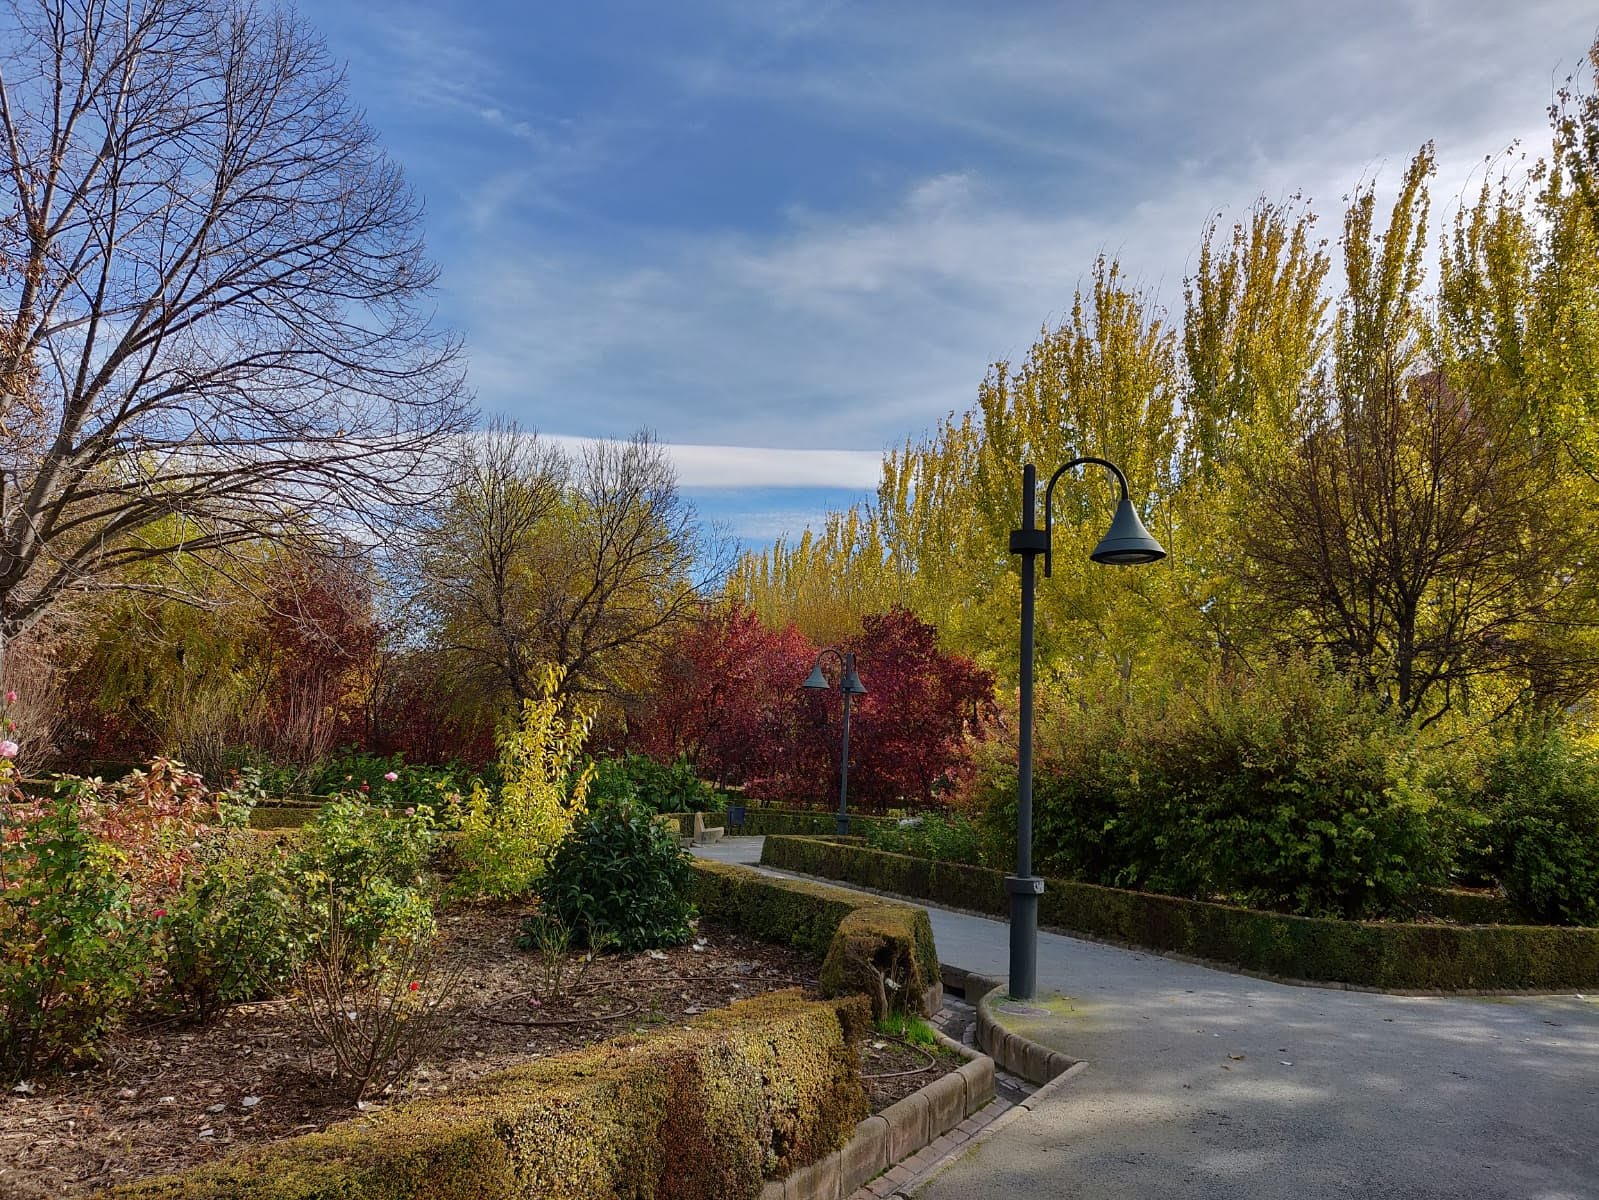
\includegraphics[width=0.5\textwidth]{Fotos/texturas.jpg}
		\end{figure}	
\end{itemize}

\begin{table}[H]
\centering
\begin{tabular}{|c|c|c|c|}
\hline
\diagbox[width=15em]{\textit{Códec}/Formato}{\\Información} & Tamaño & Valoración & Ranking \\
\hline
\textsc{bmp} & 5.8 MB & 
\includegraphics[width=0.03\textwidth]{r.png} & 2º \\ \hline
\textsc{tiff} sin compresión & 5.8 MB & 
\includegraphics[width=0.03\textwidth]{mb.png} & 1º \\ \hline
\textsc{tiff} con deflación & 4.6 MB & 
\includegraphics[width=0.03\textwidth]{mb.png} & 1º \\ \hline
\textsc{gif} & 1.6 MB & 
\includegraphics[width=0.03\textwidth]{r.png} & 2º \\ \hline
\textsc{jpeg} con calidad :100 & 1.9 MB & 
\includegraphics[width=0.03\textwidth]{mb.png} & 1º \\ \hline
\textsc{jpeg} con calidad :50 & 318.6 kB & 
\includegraphics[width=0.03\textwidth]{mb.png} & 1º \\ \hline
\textsc{jpeg} con calidad :5 & 52.4 kB & \includegraphics[width=0.03\textwidth]{mm.png} & 3º \\ \hline
\textsc{png} & 3.8 MB & \includegraphics[width=0.03\textwidth]{mb.png} & 1º \\ \hline
\end{tabular}
\caption{Imagen poco cromática}
\label{tab:my-table}
\end{table}

\subsubsection{Explicaciones a las valoraciones}
\begin{enumerate}
	\item \textsc{tiff} sin compresión y con deflación, \textsc{jpeg} con calidad 100 y 50 y \textsc{png}: en estos 5 casos, la imagen se ve perfecta: nítida, con gran cantidad de colores, con gran calidad... La imagen se mantiene tal y como se ve en la realidad.
	\item \textsc{bmp} y \textsc{gif}: en este caso, la calidad cambia bastante, ya que la imagen se ven muy oscurecida con respecto a la original.
	\item \textsc{jpeg} con calidad 5: de nuevo, la imagen se ve muy mal ya que está completamente pixelada, se pierden colores y los árboles parecen árboles del \textit{minecraft}, un juego donde el mundo es cuadrado.
\end{enumerate}

\subsubsection{Conclusión}
En este caso, debido a la gran cantidad de colores y a la intensidad de los mismos, los \textsc{códecs} \textsc{gif} y \textsc{bmp} cambian mucho con respecto a otros casos, donde, es cierto que la imagen se oscurecia pero no tan drásticamente como en este caso.

\newpage

\subsection{Imagen con texto}

Esta imagen es la primera que no es una imagen tomada por mí, sino que es una imagen textual, artificial.

\begin{itemize}
	\item Formato original: \textsc{.bmp}
	\item Tipo de imagen: texto
	\item Imagen:
		\begin{figure}[H]
		\centering
			\includegraphics[width=0.5\textwidth]{Fotos/texto.png}
		\end{figure}	
\end{itemize}

\begin{table}[H]
\centering
\begin{tabular}{|c|c|c|c|}
\hline
\diagbox[width=15em]{\textit{Códec}/Formato}{\\Información} & Tamaño & Valoración & Ranking \\
\hline
\textsc{bmp} & 480.1 kB & \includegraphics[width=0.03\textwidth]{mb.png} & 1º \\ \hline
\textsc{tiff} sin compresión & 496.1 kB & \includegraphics[width=0.03\textwidth]{mb.png} & 1º \\ \hline
\textsc{tiff} con deflación & 42.3 kB & \includegraphics[width=0.03\textwidth]{mb.png} & 1º \\ \hline
\textsc{gif} & 9.8 kB & \includegraphics[width=0.03\textwidth]{mb.png} & 1º \\ \hline
\textsc{jpeg} con calidad :100 & 52.6 kB & \includegraphics[width=0.03\textwidth]{r.png} & 2º \\ \hline
\textsc{jpeg} con calidad :50 & 24.9 kB & \includegraphics[width=0.03\textwidth]{m.png} & 3º \\ \hline
\textsc{jpeg} con calidad :5 & 16.5 kB & \includegraphics[width=0.03\textwidth]{mm.png} & 4º \\ \hline
\textsc{png} & 28.6 kB & \includegraphics[width=0.03\textwidth]{mb.png} & 1º \\ \hline
\end{tabular}
\caption{Imagen poco cromática}
\label{tab:my-table}
\end{table}

\subsubsection{Explicaciones de las valoraciones}
\begin{enumerate}
	\item \textsc{bmp}, \textsc{tiff} sin compresión y con deflación, \textsc{gif} y \textsc{png}: mantienen la calidad de la imagen original, ya que nos se ven ``manchas'' alrededor de las letras ni se ven excesivamente pixeladas cuando se aumenta mucho la imagen.
	\item \textsc{jpeg} con calidad 100: aún no se aprecian manchas ni cuadrados grises alrededor de las letras pero sí se ve un mayor pixelado al hacer zoom en la imagen.
	\item \textsc{jpeg} con calidad 50: se ven pequeños cuadrados grisáceos alrededor de las letras. Además, éstas se ven más pixeladas que antes.
	\item \textsc{jpeg} con calidad 5: se ven muchos cuadrados grises dispersos por la imagen. Todas las letras se ven muy pixeladas a simple vista. Cuesta incluso leer bien el texto.
\end{enumerate}

\subsubsection{Conclusión}

Para esta ocasión, las imágenes que han sido codificadas en \textsc{jpeg}, sin importar el grado de compresión que se le ha dado, pierden mucha calidad, ya que las letras están pixeladas, se ven manchas por toda la imagen, a veces incluso cuesta leerla... No obstante, con los demás \textit{códecs} la imagen está muy bien y solo se ven pixeles cuando se aumenta muchísimo el tamaño de la imagen (más del 400\% del zoom original).

\newpage

\subsection{Imagen gráfica}

Por último, tenemos otra imagen artificial, en este caso de un gráfico generado por ordenador, fruto de una práctica de la asignatura \textit{Informática Gráfica}, cursada en esta misma titulación.

\begin{itemize}
	\item Formato original: \textsc{.bmp}
	\item Tipo de imagen: gráfica
	\item Imagen:
		\begin{figure}[H]
		\centering
			\includegraphics[width=0.5\textwidth]{Fotos/graficos.png}
		\end{figure}	
\end{itemize}

\begin{table}[H]
\centering
\begin{tabular}{|c|c|c|c|}
\hline
\diagbox[width=15em]{\textit{Códec}/Formato}{\\Información} & Tamaño & Valoración & Ranking \\
\hline
\textsc{bmp} & 680.2 kB & \includegraphics[width=0.03\textwidth]{mb.png} & 1º \\ \hline
\textsc{tiff} sin compresión & 696.3 kB & \includegraphics[width=0.03\textwidth]{mb.png} & 1º \\ \hline
\textsc{tiff} con deflación & 52.4 kB & \includegraphics[width=0.03\textwidth]{mb.png} & 1º \\ \hline
\textsc{gif} & 14.9 kB & \includegraphics[width=0.03\textwidth]{mb.png} & 1º \\ \hline
\textsc{jpeg} con calidad :100 & 132.1 kB & \includegraphics[width=0.03\textwidth]{mb.png} & 1º \\ \hline
\textsc{jpeg} con calidad :50 & 28.5 kB & \includegraphics[width=0.03\textwidth]{m.png} & 2º \\ \hline
\textsc{jpeg} con calidad :5 & 16.7 kB & \includegraphics[width=0.03\textwidth]{mm.png} & 3º \\ \hline
\textsc{png} & 29 kB & \includegraphics[width=0.03\textwidth]{mb.png} & 1º \\ \hline
\end{tabular}
\caption{Imagen poco cromática}
\label{tab:my-table}
\end{table}

\subsubsection{Explicaciones a las valoraciones}
\begin{enumerate}
	\item \textit{bmp}, \textit{tiff} sin compresión y con deflación, \textit{gif}, \textit{jpeg} con calidad 100 y \textit{png}: en todos estos casos, la imagen se bien, solo se ven los pixeles al aumentar mucho el zoom. Pero a simple vista, la figura está nítida y clara, y los colores son los esperados.
	\item \textit{jpeg} con calidad 50: esta opción es mucho peor que las anteriores. Los píxeles se ven mucho más de cerca y la imagen se ve algo borrosa. No se conserva bien la calidad como ocurre con el mismo \textit{códec} pero con calidad 100.
	\item \textit{jpeg} con calidad 5: esta imagen se ve muy muy mal, se destacan todos los píxeles, la imagen se ve ``sucia'', con muchas manchas grises por toda la figura y ni siquiera se conservan los colores de los ejes sobre los que se sitúa la hormiga.
\end{enumerate}

\subsubsection{Conclusión}
Para esta última imagen, la mayoría de \textit{códecs}, igual que ocurrió con el texto, son válidos, ya que mantienen muy bien la calidad original de la figura que se muestra. No obstante, \textit{jpeg} con una calidad inferior a 100, es decir, donde realmente hay pérdidas durante la compresión, trata muy mal a la imagen y hace que se vea mal. Se pierde definición en los bordes, e incluso se pierden colores.

\newpage

\subsection{Conclusiones}

Como se ha podido ir comprobando durante el estudio realizado, el \textit{códec} más adecuado para cada imagen depende de la naturaleza de la propia imagen. Según la variedad de color, de texturas, la definición de los bordes, la iluminación o si la imagen es natural o artifical, el \textit{códec} utilizado influye con mucho impacto a la hora de visualizar la imagen.\\

No obstante, como se ha ido comprobando, el mejor \textit{códec} es el \textsc{tiff}, ya que es el que mejor mantiene todas las propiedades en todas las imágenes, en concreto el mejor es el \textsc{tiff} con deflación ya que los requerimientos de disco para imágenes comprimidas así son menores; no obstante, el formato \textsc{tiff} (al menos con las dos variantes que yo he utilizado), comprime más bien poco, y deja imágenes de gran tamaño, mientras que formatos como \textsc{jpeg} o incluso \textsc{png} o \textsc{gif} quizá no mantengan la calidad tan alta pero utilizan una cantidad de memoria considerablemente menor.\\

Por tanto, y como conclusión final, podría decir que el mejor \textit{códec} es el \textsc{tiff} pero que a su vez, es el que requiere de una mayor cantidad de espacio en disco. La pregunta es, ¿prima la calidad sobre el espacio ocupado, o es al revés? Esa pregunta quizá dependa de la cantidad de espacio de la que dispongamos y del uso que le demos a cada fotografía.

\newpage

\section{Software utilizado}

Para poder cambiar los distintos \textit{códecs} y variar sus parámetros de compresión, se ha utilizado \textbf{\textit{darktable}}, una aplicación de escritorio que permite modificar una enorme cantidad de parámetros de las imágenes, que muestra el histograma de cada una y que tiene dos posibilidades: utilizar el cuarto oscuro, donde se pueden modificar unos atributos concretos de las imágenes, o utilizar la mesa de luz, donde se pueden modificar otros.\\

\begin{itemize}
	\item \textcolor{blue}{\url{https://www.darktable.org/}}
\end{itemize}

\section{Bibliografía}

\begin{itemize}
	\item Transparencias de teoría de Sistemas Multimedia: la imagen
	\item \textcolor{blue}{\url{https://www.darktable.org/usermanual/en/}}
	\item \textcolor{blue}{\url{https://opensource.com/life/16/4/how-use-darktable-digital-darkroom}}
\end{itemize}

\section{Enlaces de interés}

Las imágenes utilizadas para el estudio, con los distintos \textit{códecs} y distintos parámetros se encuentran en el enlace aportado abajo. Los nombres de los archivos corresponden a las siguientes modificaciones (donde \textit{x} es el nombre de la imagen en particular):

\begin{itemize}
	\item \textsc{x.bmp} = imagen en formato \textsc{bmp}.
	\item \textsc{xsin.tif} = imagen en formato \textsc{tif} sin compresión.
	\item \textsc{xdef.tif} = imagen en formato \textsc{tif} con deflación.
	\item \textsc{x.gif} = imagen en formato \textsc{gif}.
	\item \textsc{x100.jpg} = imagen en formato \textsc{jpeg} con calidad 100.
	\item \textsc{x50.jpg} = imagen en formato \textsc{jpeg} con calidad 50.
	\item \textsc{x5.jpg} = imagen en formato \textsc{jpeg} con calidad 5.
	\item \textsc{x.png} = imagen en formato \textsc{png}.
\end{itemize}

\footnotesize{\textcolor{blue}{\url{https://drive.google.com/drive/folders/167FG6zSFZ_Kf2PR5Bgbe2HG5bkr4Cg4K?usp=sharing}}}

\end{document}